\documentclass[a4paper,12pt]{article}
\usepackage{mypreamble}

%% Page setup
\geometry{
    margin=2cm,
    includehead,
    % includefoot,
    headsep=\baselineskip,
}
\pagestyle{fancy}
\fancyfoot{}
\MakeDoubleHeader% {<l1>}{<l2>}{<r1>}{<r2>}
    {\TextHomeworkEng~\#6}
    {Automata Theory}
    {\TextDiscreteMathEng}
    {\IconSpring~Spring 2024}

%% Add custom setup below

%% BNF grammar
\usepackage{syntax}

%% TikZ
\usetikzlibrary{automata,shapes}
\tikzset{
    position/.style args={#1:#2 from #3}{
        at=(#3.#1), anchor=#1+180, shift=(#1:#2)
    },
    dot/.style={
        draw,
        fill=black,
        shape=circle,
        minimum size=4pt,
        inner sep=0pt,
        outer sep=0pt,
    },
}
\tikzstyle{mygraphstyle}=[
    auto,
    on grid,
]
\tikzstyle{myautomatonstyle}=[
    auto, on grid,
    >={Stealth[]},
    shorten >=1pt,
    semithick,
    bend angle=15,
    initial text={},
    every state/.style={
        inner sep=0pt,
        minimum size=2em,
    },
]

%% Theorems
\declaretheoremstyle[
    spaceabove=6pt,
    spacebelow=6pt,
    postheadspace=0.5em,
    notefont=\normalfont\scshape,
]{mystyle}
\declaretheorem[style=mystyle]{theorem}


\begin{document}
\selectlanguage{english}

\begin{tasks}

    \item For each given regular expression~$P$, construct a DFA (Deterministic Finite Automaton), and find the number of accepted word of length at most~5, i.e. the size of the set $\mathcal{L}' =\nobreak \Set{w \in\nobreak \mathcal{L}(P) \given |w| \leq 5}$.
    For \enquote{any} (\verb/./) and \enquote{negative} (\verb/[^.]/) matches, assume that the alphabet is $\Sigma = \Set{\texttt{a}, \texttt{b}, \texttt{c}, \texttt{d}}$.

    \begin{multicols}{3}
    \begin{subtasks}
        \item $P_{\arabic{subtasksi}} = \verb/ab*/$
        \item $P_{\arabic{subtasksi}} = \verb/a+b?c/$
        \item $P_{\arabic{subtasksi}} = \verb/[^cd]+c{3}/$
        \item $P_{\arabic{subtasksi}} = \verb/[^a](.|ddd)?/$
        \item $P_{\arabic{subtasksi}} = \verb/d(a|bc)*/$
        \item $P_{\arabic{subtasksi}} = \verb/((a|ab)[cd]){2}/$
    \end{subtasks}
    \end{multicols}


    \item Describe the set of strings defined by each of these sets of productions in EBNF\Href{https://en.wikipedia.org/wiki/Backus-Naur_form} (extended Backus-Naur form).

    \begin{multicols}{2}
    \begin{subtasks}
        \setlength{\grammarparsep}{0pt plus 4pt}
        \setlength{\grammarindent}{5em}

        \item \begin{grammar}
            <string> ::= <L>+ <D>? <L>+

            <L> ::= "a" | "b" | "c"

            <D> ::= "0" | "1"
        \end{grammar}

        \item \begin{grammar}
            <string> ::= <sign>? <N>

            <sign> ::= `+' | `-'

            <N> ::= <D> (<D> | "0")*

            <D> ::= "1" | $\ldots$ | "9"
        \end{grammar}

        \item \begin{grammar}
            <string> ::= <L>* (<D>+)? <L>*

            <L> ::= "x" | "y"

            <D> ::= "0" | "1"
        \end{grammar}

        \item \begin{grammar}
            <string> ::= <C> <R>*

            <C> ::= "a" | $\ldots$ | "z" | "A" | $\ldots$ | "Z"

            <D> ::= "0" | $\ldots$ | "9"

            <R> ::= <C> | <D> | `_'
        \end{grammar}
    \end{subtasks}
    \end{multicols}


    \item Let $\mathcal{G} = \Pair{V, T, S, P}$ be the phrase-structure grammar with vocabulary $V = \Set{\mathtt{A}, \mathtt{S}}$, terminal symbols $T = \Set{0, 1}$, start symbol $S = \mathtt{S}$, and set of productions $P$: $\mathtt{S} \to \mathtt{1S}$, $\mathtt{S} \to \mathtt{00A}$, $\mathtt{A} \to \mathtt{0A}$, $\mathtt{A} \to \mathtt{0}$.

    \begin{subtasks}
        \item Show that \texttt{111000} belongs to the language generated by $\mathcal{G}$.
        \item Show that \texttt{11001} does not belong to the language generated by $\mathcal{G}$.
        \item What is the language generated by $\mathcal{G}$?
    \end{subtasks}


    \item Find the output generated from the input string \texttt{01110} for each of the following Mealy machines.

    \tikz[myautomatonstyle,baseline=(xxx.base)]{
        \node[state, initial] (s0) {$s_0$};
        \node[state, right=2.5cm of s0] (s1) {$s_1$};
        \node[state, below=2.5cm of s0] (s2) {$s_2$};
        \node[state, right=2.5cm of s2] (s3) {$s_3$};
        \coordinate (xxx) at ($(s0)!.5!(s2)$);
        \path[->]
            (s0) edge [bend left, above] node {0/1} (s1)
            (s1) edge [bend left, below] node {0/1} (s0)
            (s0) edge [bend right, left] node {1/0} (s2)
            (s2) edge [bend right, right] node {1/0} (s0)
            (s1) edge [bend left, right] node {1/0} (s3)
            (s3) edge [bend left, left] node {0/1} (s1)
            (s2) edge [bend left, above] node {0/0} (s3)
            (s3) edge [bend left, below] node {1/1} (s2)
        ;
    }%
    \hfill%
    \tikz[myautomatonstyle,baseline=(xxx.base)]{
        \node[state, initial] (s0) {$s_0$};
        \node[state, above right=1cm and 2cm of s0] (s1) {$s_1$};
        \node[state, below right=1cm and 2cm of s0] (s2) {$s_2$};
        \coordinate (xxx) at (s0);
        \path[->]
            (s0) edge [bend left, above, sloped] node {0/0} (s1)
            (s0) edge [bend left, above, sloped] node {1/1} (s2)
            (s1) edge [loop right, above, near start] node {1/0} (s1)
            (s1) edge [] node {0/0} (s2)
            (s2) edge [loop right, above, near start] node {0/1} (s2)
            (s2) edge [bend left, below, sloped] node {1/0} (s0)
        ;
    }%
    \hfill%
    \tikz[myautomatonstyle,baseline=(xxx.base)]{
        \node[state, initial] (s0) {$s_0$};
        \node[state, right=2.5cm of s0] (s1) {$s_1$};
        \node[state, below=2.5cm of s0] (s2) {$s_2$};
        \node[state, right=2.5cm of s2] (s3) {$s_3$};
        \coordinate (xxx) at ($(s0)!.5!(s2)$);
        \path[->]
            (s0) edge [bend left, above] node {1/1} (s1)
            (s1) edge [bend left, below] node {0/0} (s0)
            (s1) edge [loop right, midway, right] node {1/1} (s1)
            (s0) edge [above, sloped, near end] node {0/0} (s3)
            (s2) edge [above, sloped, near start] node {1/1} (s1)
            (s2) edge [below] node {0/0} (s3)
            (s3) edge [right] node {0/0} (s1)
            (s3) edge [loop right, midway, right] node {1/0} (s3)
        ;
    }


    \item Construct a Moore machine for each of the following descriptions.

    \begin{subtasks}
        \item Determine the residue modulo~3 of the input treated as a binary number.
        For example, for input $\varepsilon$ (which corresponds to \enquote{value} 0) the residue is 0; \texttt{101} (5 in decimal) has residue 2; and \texttt{1010} (value 10) has residue 1.

        \item Output the residue modulo~5 of the input from $\Set{0,1,2}^*$ treated as a ternary (base~3) number.

        \item Output $A$ if the binary input ends with \texttt{101}; output $B$ if it ends with \texttt{110}; otherwise output~$C$.
    \end{subtasks}


    \item Show that regular languages are \emph{closed} under the following operations.

    \begin{subtasks}
        \item Union, that is, if $L_1$ and $L_2$ are regular languages, then $L_1 \union L_2$ is also regular.
        \item Concatenation, that is, if $L_1$ and $L_2$ are regular languages, then $L_1 \cdot L_2$ is also regular.
        \item Kleene star, that is, if $L$ is a regular language, then $L^*$ is also regular.
        \item Complement, that is, if $L$ is a regular language, then $\overline{L} = \Sigma^* - L$ is also regular.
        \item Intersection, that is, if $L_1$ and $L_2$ are regular languages, then $L_1 \intersection L_2$ is also regular.
    \end{subtasks}


    \newpage

    \item Determine whether the following languages are regular or not. For non-regular languages, use Pumping lemma to prove that they are not regular. For each regular language, provide a regular expression and construct an $\varepsilon$-NFA.

    \begin{subtasks}
        \item $L_{\arabic{subtasksi}} = \Set{w \in \Set{0, 1}^* \given \text{length of $w$ is odd}}$

        \item $L_{\arabic{subtasksi}} = \Set{0^n 1^n \given n \in \Natural}$

        \item $L_{\arabic{subtasksi}} = \Set{w \in \Set{0, 1}^* \given \text{$w$ contains an even number of 1s}}$

        \item $L_{\arabic{subtasksi}} = \Set{1^{n^2} \given n \in \Natural}$
    \end{subtasks}


    \item Consider a finite-state automaton $M = (\Sigma, Q, q_0, F, \delta)$ and a non-negative integer~$k$.
    Let $R_k$ be the relation on the set of states of $M$ such that $s \mathrel{R_k} t$ if and only if for every input string $w \in \Sigma^*$ with $|w| \leq k$, $\delta(s, w)$ and $\delta(t, w)$ are both final states or both not final states.
    Furthermore, let $R^*$ be the relation on the set of states of $M$ such that $s \mathrel{R^*} t$ if and only if for every input string $w \in \Sigma^*$, regardless of length, $\delta(s, w)$ and $\delta(t, w)$ are both final states or both not final states.

    \begin{subtasks}
        \item Show that for every nonnegative integer~$k$, $R_k$ is an equivalence relation on~$S$.
        \par Two states $s$ and $t$ are called $k$-equivalent if $s \mathrel{R_k} t$.

        \item Show that $R^*$ is an equivalence relation on $S$.
        \par Two states $s$ and $t$ are called $*$-equivalent if $s \mathrel{R^*} t$.

        \item Show that if two states $s$ and $t$ are $k$-equivalent ($k > 0$), then they are also $(k - 1)$-equivalent.

        \item Show that the equivalence classes of $R_k$ are a \emph{refinement} of the equivalence classes of $R_{k-1}$.

        \item Show that if two states $s$ and $t$ are $k$-equivalent for every non-negative integer $k$, then they are $*$-equivalent.

        \item Show that all states in a given $R^*$-equivalence class are final or all are not final.

        \item Show that if two states $s$ and $t$ are $*$-equivalent, then $\delta(s, a)$ and $\delta(t, a)$ are also $*$-equivalent for all $a \in \Sigma$.
    \end{subtasks}


    \item Consider the finite-state automaton $M = (\Sigma, Q, q_0, F, \delta)$ depicted below.

    \tikz[myautomatonstyle]{
        \node[state, initial] (s0) {$s_0$};
        \node[state, above right=1cm and 2cm of s0] (s1) {$s_1$};
        \node[state, below right=1cm and 2cm of s0] (s2) {$s_2$};
        \node[state, accepting, right=2cm of s1] (s3) {$s_3$};
        \node[state, right=2cm of s2] (s4) {$s_4$};
        \node[state, right=2cm of s3] (s5) {$s_5$};
        \node[state, accepting, right=2cm of s4] (s6) {$s_6$};

        \path[->]
            (s0) edge [above, sloped] node {0} (s1)
                 edge [below, sloped] node {1} (s2)
            (s1) edge [above] node {0} (s3)
                 edge [above, sloped] node {1} (s4)
            % (s2) edge [above, sloped, very near start] node {0} (s5)
            (s2) edge [out=-40, in=-140, below] node {1} (s6)
            (s3) edge [loop above, right, near end] node {0} (s3)
                 edge [left] node {1} (s4)
            (s4) edge [bend right, below, sloped, near start] node {0} (s5)
                 edge [below] node {1} (s6)
            (s5) edge [above] node {0} (s3)
                 edge [bend right, above, sloped, near start] node {1} (s4)
            (s6) edge [above, sloped, very near start] node {0} (s3)
                 edge [loop right, right] node {1} (s6)
        ;
        \draw[->] (s2)
            to[out=45, in=-80] node [above, sloped, near start] {0} ++(0.7, 2)
            to[out=100, in=180] ++(1.3,1.4)
            to[out=0, in=120] (s5)
        ;
    }

    \begin{subtasks}
        \item Find the $k$-equivalence classes of $M$ for $k = 0, 1, 2, 3$.

        \item Find the $*$-equivalence classes of $M$.

        \item Construct the quotient automaton $\overline{M}$ of $M$.

        $\triangleright$ The quotient automaton $\overline{M}$ of the deterministic finite-state automaton $M = (\Sigma, S, s_0, F, \delta)$ is the finite state automaton $\overline{M} = (\Sigma, \overline{S}, [s_0]_{R^*}, \overline{F}, \overline{\delta})$, where the set of states $\overline{S}$ is the set of $R^*$-equivalence classes of $S$; the transition function $\overline{\delta}$ is defined by $\overline{\delta}([s]_{R^*}, a) = [\delta(s, a)]_{R^*}$ for all states $[s]_{R^*}$ of $\overline{M}$ and input symbols $a \in \Sigma$; and $\overline{F}$ is the set consiting of $R^*$-equivalence classes of final states of $M$.
    \end{subtasks}


    \newpage

    \item Solve the following regex crosswords\footnote{Credits: \url{https://regexcrossword.com}}.
    Fill each cell with a single ASCII character (an uppercase letter, a digit, a punctuation mark, or a space).
    Each row/column, when read left to right or top to bottom must match the regular expression(s) given for that row/column.

    % Beginner > Beatles
    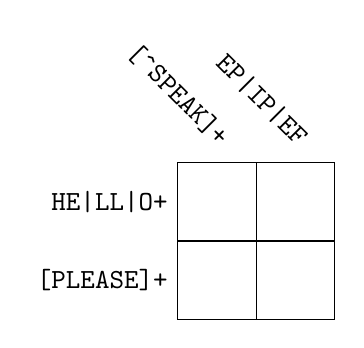
\begin{tikzpicture}[baseline=0]
        \draw (0,0) grid (2,-2);
        \node at (0, -0.5) [left] {\verb/HE|LL|O+/};
        \node at (0, -1.5) [left] {\verb/[PLEASE]+/};
        \node at (0.5, 0) [rotate=-45, above left] {\verb/[^SPEAK]+/};
        \node at (1.5, 0) [rotate=-45, above left] {\verb/EP|IP|EF/};
    \end{tikzpicture}%
    \hfill%
    %
    % Experienced > Royal Dinner
    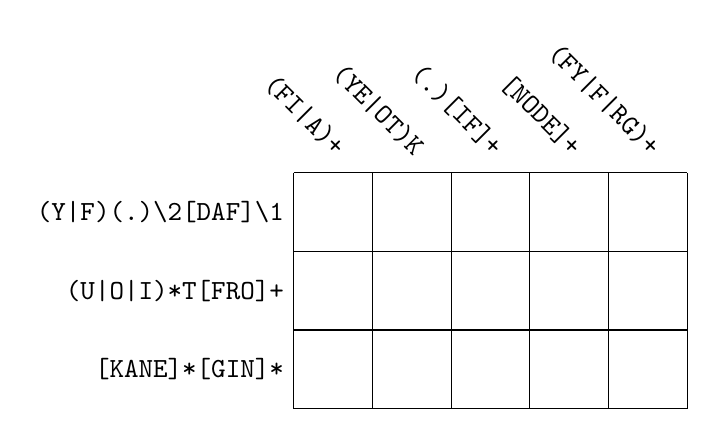
\begin{tikzpicture}[baseline=0]
        \draw (0,0) grid (5,-3);
        \node at (0, -0.5) [left] {\verb/(Y|F)(.)\2[DAF]\1/};
        \node at (0, -1.5) [left] {\verb/(U|O|I)*T[FRO]+/};
        \node at (0, -2.5) [left] {\verb/[KANE]*[GIN]*/};
        \node at (0.5, 0) [rotate=-45, above left] {\verb/(FI|A)+/};
        \node at (1.5, 0) [rotate=-45, above left] {\verb/(YE|OT)K/};
        \node at (2.5, 0) [rotate=-45, above left] {\verb/(.)[IF]+/};
        \node at (3.5, 0) [rotate=-45, above left] {\verb/[NODE]+/};
        \node at (4.5, 0) [rotate=-45, above left] {\verb/(FY|F|RG)+/};
    \end{tikzpicture}

    % Intermediate > Technology
    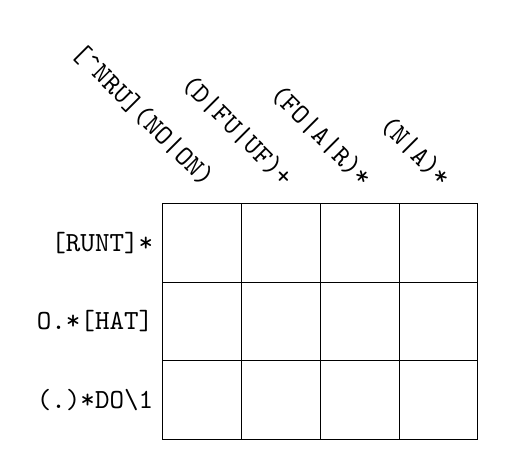
\begin{tikzpicture}[baseline=0]
        \draw (0,0) grid (4,-3);
        \node at (0, -0.5) [left] {\verb/[RUNT]*/};
        \node at (0, -1.5) [left] {\verb/O.*[HAT]/};
        \node at (0, -2.5) [left] {\verb/(.)*DO\1/};
        \node at (0.5, 0) [rotate=-45, above left] {\verb/[^NRU](NO|ON)/};
        \node at (1.5, 0) [rotate=-45, above left] {\verb/(D|FU|UF)+/};
        \node at (2.5, 0) [rotate=-45, above left] {\verb/(FO|A|R)*/};
        \node at (3.5, 0) [rotate=-45, above left] {\verb/(N|A)*/};
    \end{tikzpicture}%
    \hfill%
    %
    % Double Cross > GMC Vandura
    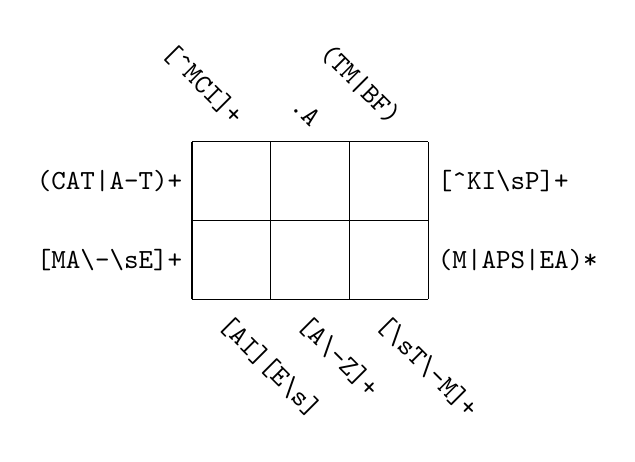
\begin{tikzpicture}[baseline=0]
        \draw (0,0) grid (3,-2);
        \node at (0, -0.5) [left] {\verb/(CAT|A-T)+/};
        \node at (0, -1.5) [left] {\verb/[MA\-\sE]+/};
        \node at (3, -0.5) [right] {\verb/[^KI\sP]+/};
        \node at (3, -1.5) [right] {\verb/(M|APS|EA)*/};
        \node at (0.5, 0) [rotate=-45, above left] {\verb/[^MCI]+/};
        \node at (1.5, 0) [rotate=-45, above left] {\verb/.A/};
        \node at (2.5, 0) [rotate=-45, above left] {\verb/(TM|BF)/};
        \node at (0.5, -2) [rotate=-45, below right] {\verb/[AI][E\s]/};
        \node at (1.5, -2) [rotate=-45, below right] {\verb/[A\-Z]+/};
        \node at (2.5, -2) [rotate=-45, below right] {\verb/[\sT\-M]+/};
    \end{tikzpicture}

    % Double Cross > Big Mac
    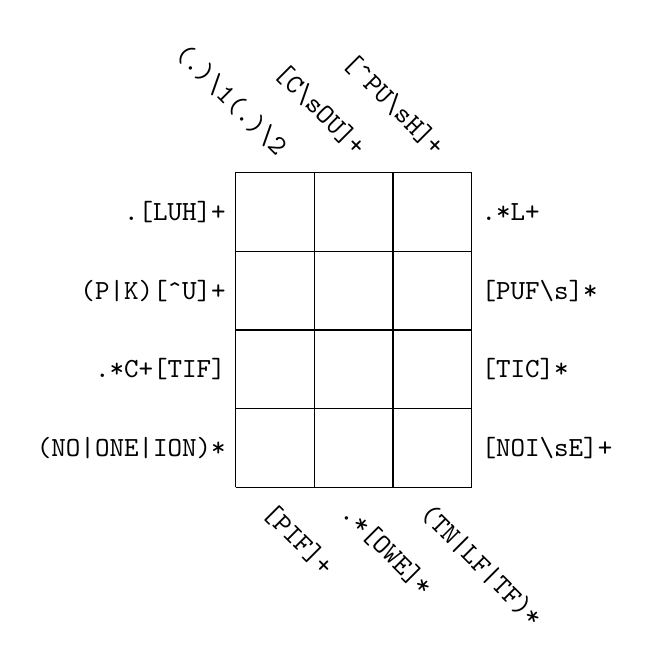
\begin{tikzpicture}[baseline=0]
        \draw (0,0) grid (3,-4);
        \node at (0, -0.5) [left] {\verb/.[LUH]+/};
        \node at (0, -1.5) [left] {\verb/(P|K)[^U]+/};
        \node at (0, -2.5) [left] {\verb/.*C+[TIF]/};
        \node at (0, -3.5) [left] {\verb/(NO|ONE|ION)*/};
        \node at (3, -0.5) [right] {\verb/.*L+/};
        \node at (3, -1.5) [right] {\verb/[PUF\s]*/};
        \node at (3, -2.5) [right] {\verb/[TIC]*/};
        \node at (3, -3.5) [right] {\verb/[NOI\sE]+/};
        \node at (0.5, 0) [rotate=-45, above left] {\verb/(.)\1(.)\2/};
        \node at (1.5, 0) [rotate=-45, above left] {\verb/[C\sOU]+/};
        \node at (2.5, 0) [rotate=-45, above left] {\verb/[^PU\sH]+/};
        \node at (0.5, -4) [rotate=-45, below right] {\verb/[PIF]+/};
        \node at (1.5, -4) [rotate=-45, below right] {\verb/.*[OWE]*/};
        \node at (2.5, -4) [rotate=-45, below right] {\verb/(TN|LF|TF)*/};
    \end{tikzpicture}%
    \hfill%
    %
    % Palindromeda > Time Walker
    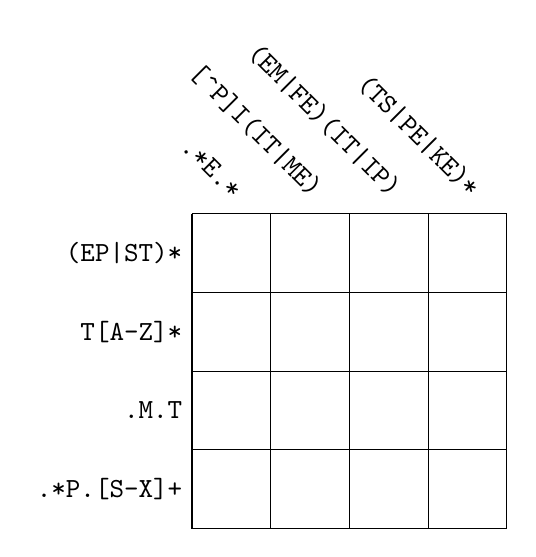
\begin{tikzpicture}[baseline=0]
        \draw (0,0) grid (4,-4);
        \node at (0, -0.5) [left] {\verb/(EP|ST)*/};
        \node at (0, -1.5) [left] {\verb/T[A-Z]*/};
        \node at (0, -2.5) [left] {\verb/.M.T/};
        \node at (0, -3.5) [left] {\verb/.*P.[S-X]+/};
        \node at (0.5, 0) [rotate=-45, above left] {\verb/.*E.*/};
        \node at (1.5, 0) [rotate=-45, above left] {\verb/[^P]I(IT|ME)/};
        \node at (2.5, 0) [rotate=-45, above left] {\verb/(EM|FE)(IT|IP)/};
        \node at (3.5, 0) [rotate=-45, above left] {\verb/(TS|PE|KE)*/};
    \end{tikzpicture}
    %
    % % Palindromeda > Ten o'clock
    % \begin{tikzpicture}[baseline=0]
    %     \draw (0,0) grid (3,-3);
    %     \node at (0, -0.5) [left] {\verb/(T|E|N)*/};
    %     \node at (0, -1.5) [left] {\verb/(.)*W+\1/};
    %     \node at (0, -2.5) [left] {\verb/[LENT]*/};
    %     \node at (0.5, 0) [rotate=-45, above left] {\verb/(ENT|NTE|NET)*/};
    %     \node at (1.5, 0) [rotate=-45, above left] {\verb/[WEAR]*/};
    %     \node at (2.5, 0) [rotate=-45, above left] {\verb/[R-Z]E*[M-R]/};
    % \end{tikzpicture}

\end{tasks}
\end{document}
